
\begin{frame}[t,plain]
\titlepage
\end{frame}

\begin{frame}{Agenda}
\tableofcontents
\end{frame}



\section{Introduction}
\subsection{Sokoban}
% sokoban intro


\begin{frame}{Introduction}{Sokoban}
  \begin{center}
    % Level 1/05 
    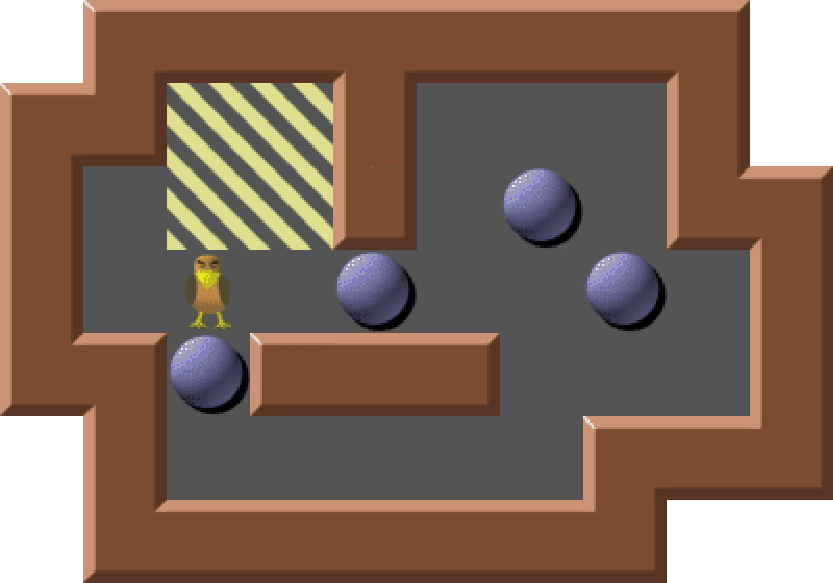
\includegraphics[height=0.7\textheight]{level.pdf}
  \end{center}
\end{frame}


\section{Heuristics}
\subsection{Combining Heuristics}
\begin{frame}{Heuristics}{Combining Heuristics}
    \begin{itemize}
    \item Pros
      \begin{itemize}
      \item Flexible
      \item Reduce code duplication
      %\item Estimate not linear
      \end{itemize}
    \item Cons
      \begin{itemize}
      \item Estimate $\neq$ actual number of steps\\
      %\item Estimate not linear
      \end{itemize}
    \end{itemize}

    \begin{itemize}
    \item Combiners
      \begin{itemize}
      \item Multiplier
      \item Adder
      \end{itemize}

    \item Example: $ A(+\{*\{B,B,a,a\},c,4\})$

    \end{itemize}
\end{frame}

\subsection{Examples}

\begin{frame}{Heuristics}{Examples: Pattern Detection}
  \begin{itemize}
  \item Illegal state ellimination
  \end{itemize}
  \begin{center}
    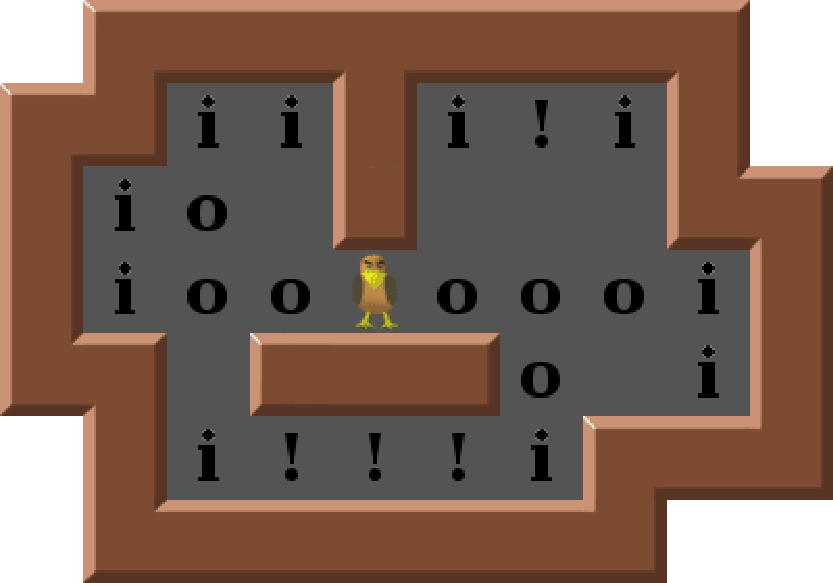
\includegraphics[height=0.7\textheight]{cornermarkings.pdf}
  \end{center}
\end{frame}

\begin{frame}{Heuristics}{Examples: Shortest Path}
  \begin{itemize}
  \item Shortest path. Calculated once for a map.
  \end{itemize}
  \begin{center}
    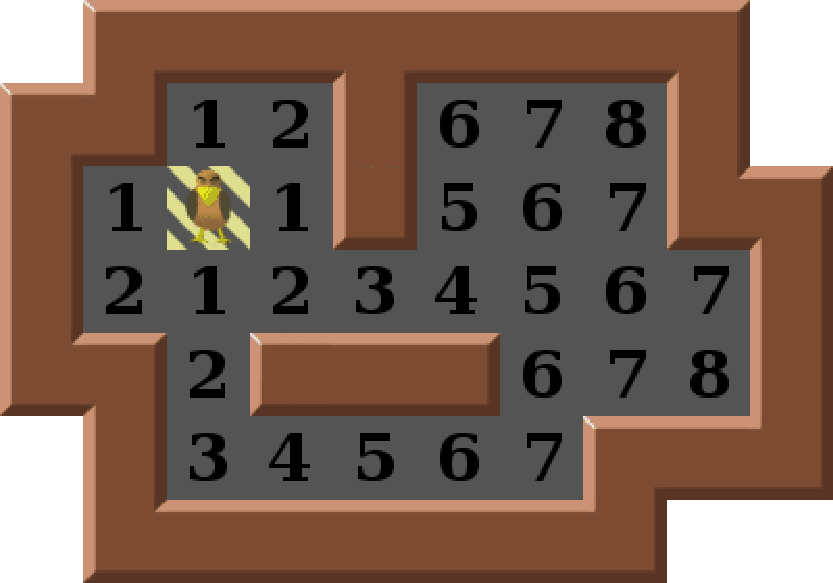
\includegraphics[height=0.5\textheight]{distances.pdf}
  \end{center}
  \begin{itemize}
  \item More heuristics. Not mentioned here.
  \end{itemize}
\end{frame}


\section{Results}
\subsection{Solution Performance}
\begin{frame}{Results}{Solution Performance}

  \begin{table}
    \centering
    \begin{tabular}{lrr}\toprule
      \textbf{ Name } & \textbf{  Time} &  \textbf{ Sol. len. }\\\midrule
      $BFSolver $&                 20147  &       0\\
      $A(i)$    &                 20058  &       0\\
      $A(c)$     &                20034  &       0\\
      $A(+\{c,i\})$ &               20000  &       0\\
      $A(+\{c,i,4\})$&              20025  &       0\\
      $A(+\{*\{i,i\},c,4\})$ &         1930  &     143\\
      $A(+\{*\{s,s\},c,4\})$  &         309  &     145\\
      $A(+\{*\{B,B,s,s\},c,4\})$&       191  &     145\\
      $A(+\{*\{B,B,a,a\},c,4\})$ &      183  &     145\\
      $A(rand)$               &   20031  &       0\\
      \bottomrule
    \end{tabular}
  \end{table}
  
\end{frame}


\subsection{State Space Growth}
\begin{frame}{Results}{State Space Growth}
  \vspace{-1cm}
  \begin{center}
    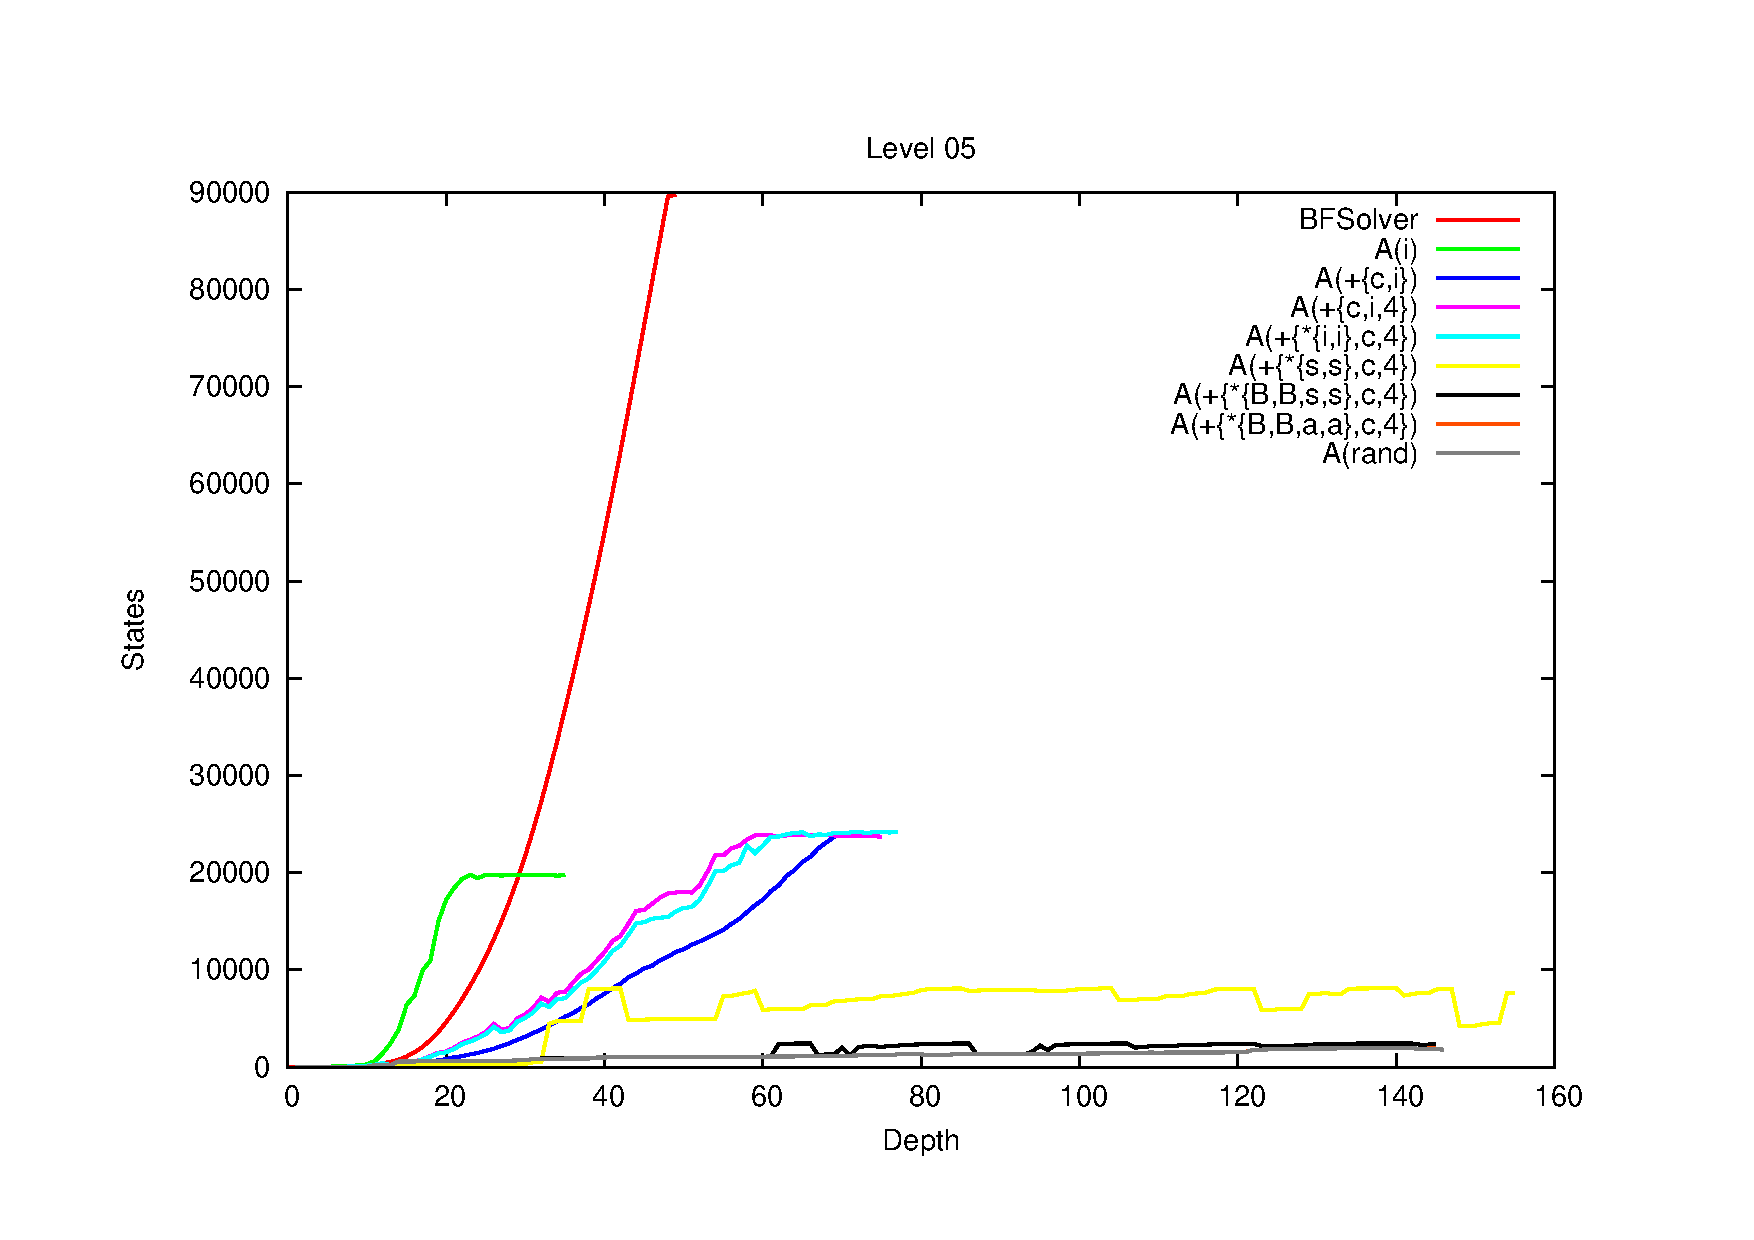
\includegraphics[height=0.93\textheight]{statespace1}
  \end{center}
\end{frame}

\begin{frame}{Results}{State Space Growth}
  \vspace{-1cm}
  \begin{center}
    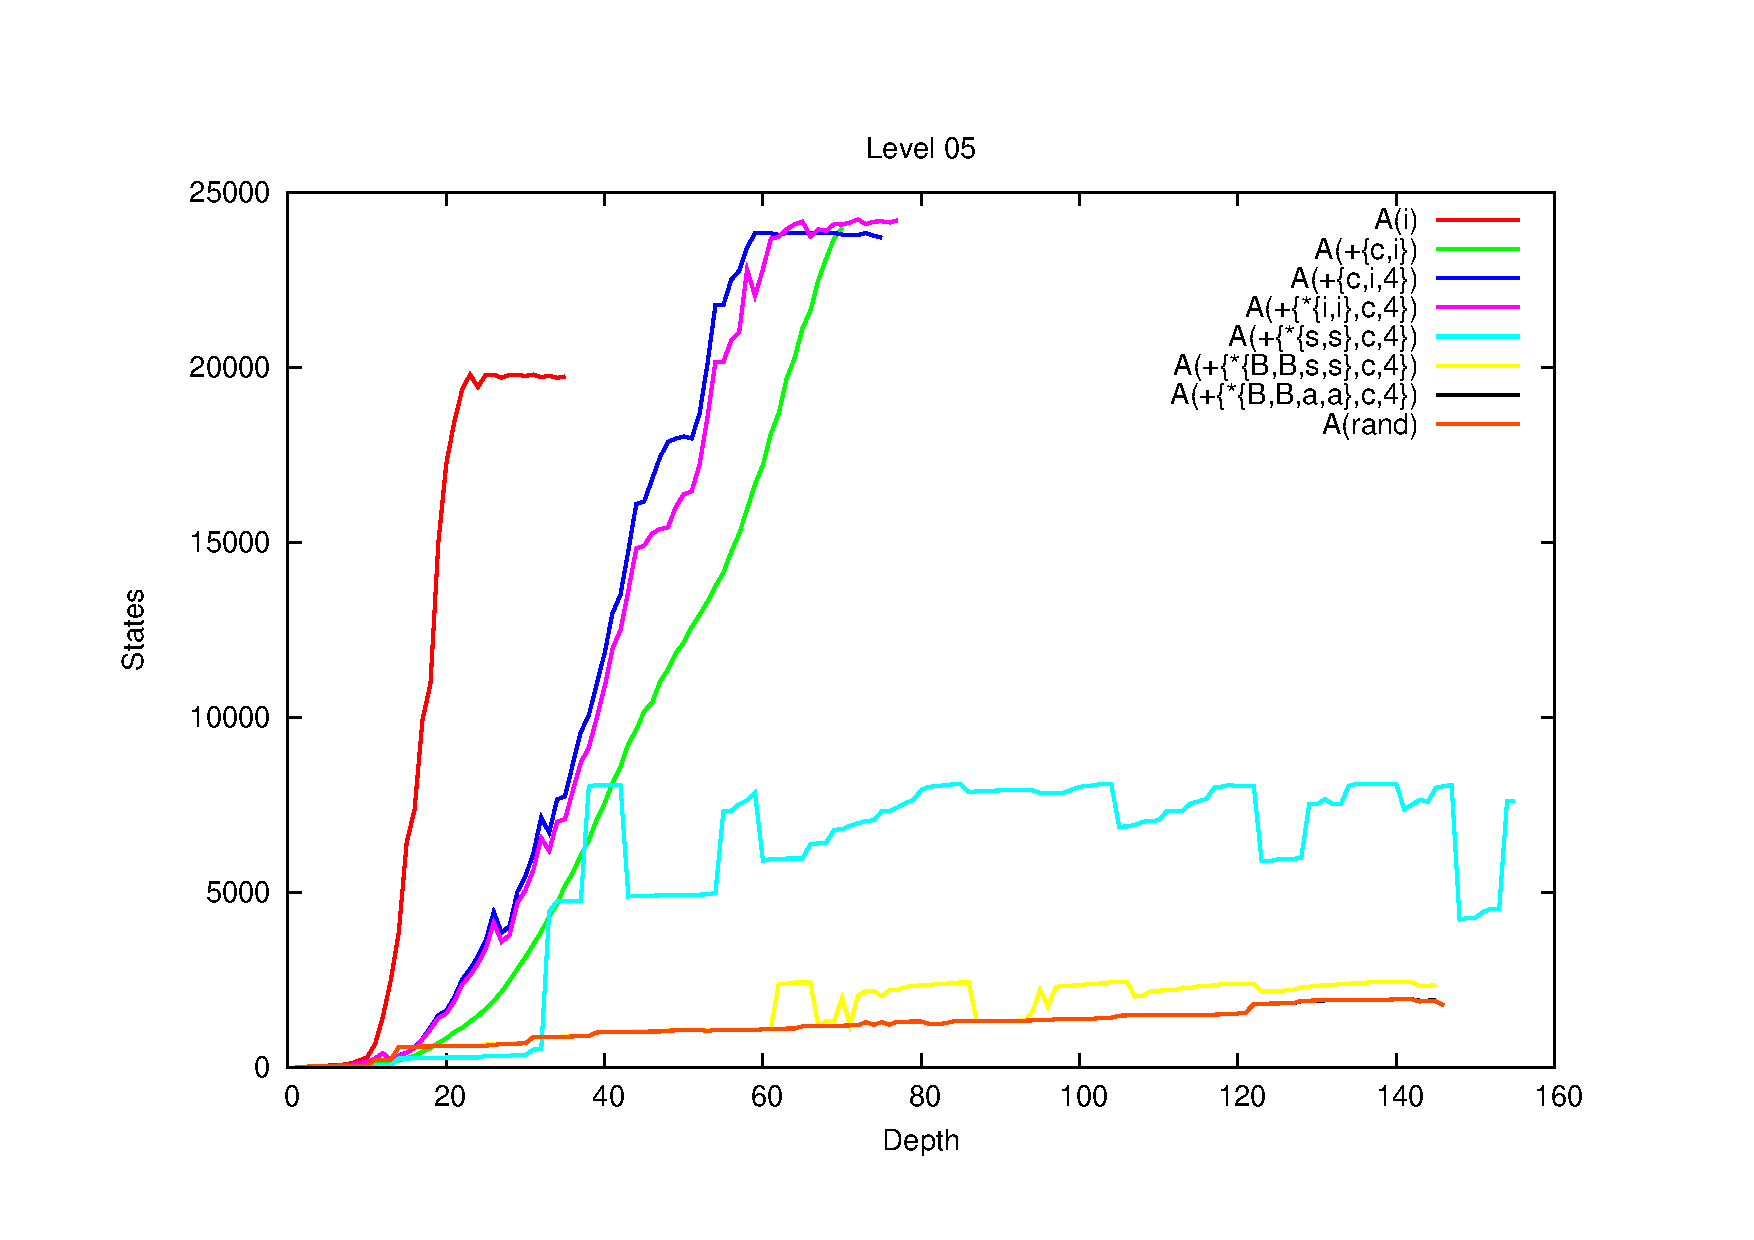
\includegraphics[height=0.93\textheight]{statespace2}
  \end{center}
\end{frame}


\section{Demonstration}

\begin{frame}{Demonstration}
  \begin{center}
    \begin{itemize}
    \item Start it up!
    \end{itemize}
  \end{center}
\end{frame}

\section{Summary}
\begin{frame}{Summary}
    \begin{itemize}
    \item Combining heuristics $\implies$ 
      \begin{itemize}
      \item Effective heuristics
      \item Easy to experiment with
      \end{itemize}
    \end{itemize}


    \begin{itemize}
        
    \item Fast and efficient solver
      \begin{itemize}
      \item Can solve 100+ steps in $\leq$ 1 second.
      \end{itemize}
      

    \end{itemize}

\end{frame}